\chapter{RESULTS}

Some of the results of this project were already discussed. These results include the implementation of a flocking algorithm in OpenCL GPU language discussed in Section~\ref{flocksection}, and the developed of the UI modifier for the Blender Game Engine. As discussed in Section~\ref{modifiersection}. This chapter will focus on showing demonstrations of the flocking rules by themselves and a demonstrations of the RTPS modifier. 

\section{Demos}

\subsection{Symmetry of the Basic Rules}
If using the \textit{separation} or \textit{cohesion} rule by themselves, meaning that only separation would have a weight constant greater than zero or only cohesion would have a weight constant greater than zero. By doing this it can be seen that these two behaviors are symmetric. Figure~\ref{alignRule} show the initial conditions in this Demo. Here are 144 boids centralized in a $5$x$5$x$5$ box. Figure~\ref{sepRule} shows two screenshots of the boids trying to spread out symmetrically. A weight of $1$ was used for separation. The, Figure~\ref{cohRule} shows four screenshots of the cohesion rule, also a weight of $1$ was used for cohesion. Since, the rendering methods that are available at this moment in RTPS are points, sprites, and screen space we are not able to present a demo on the symmetry of alignment but it is quite obvious that alignment is symmetric since we start with a velocity equal to zero, therefore all boids will be pointing to the same direction.

% alignment
\begin{figure}[htbp]
\begin{center}
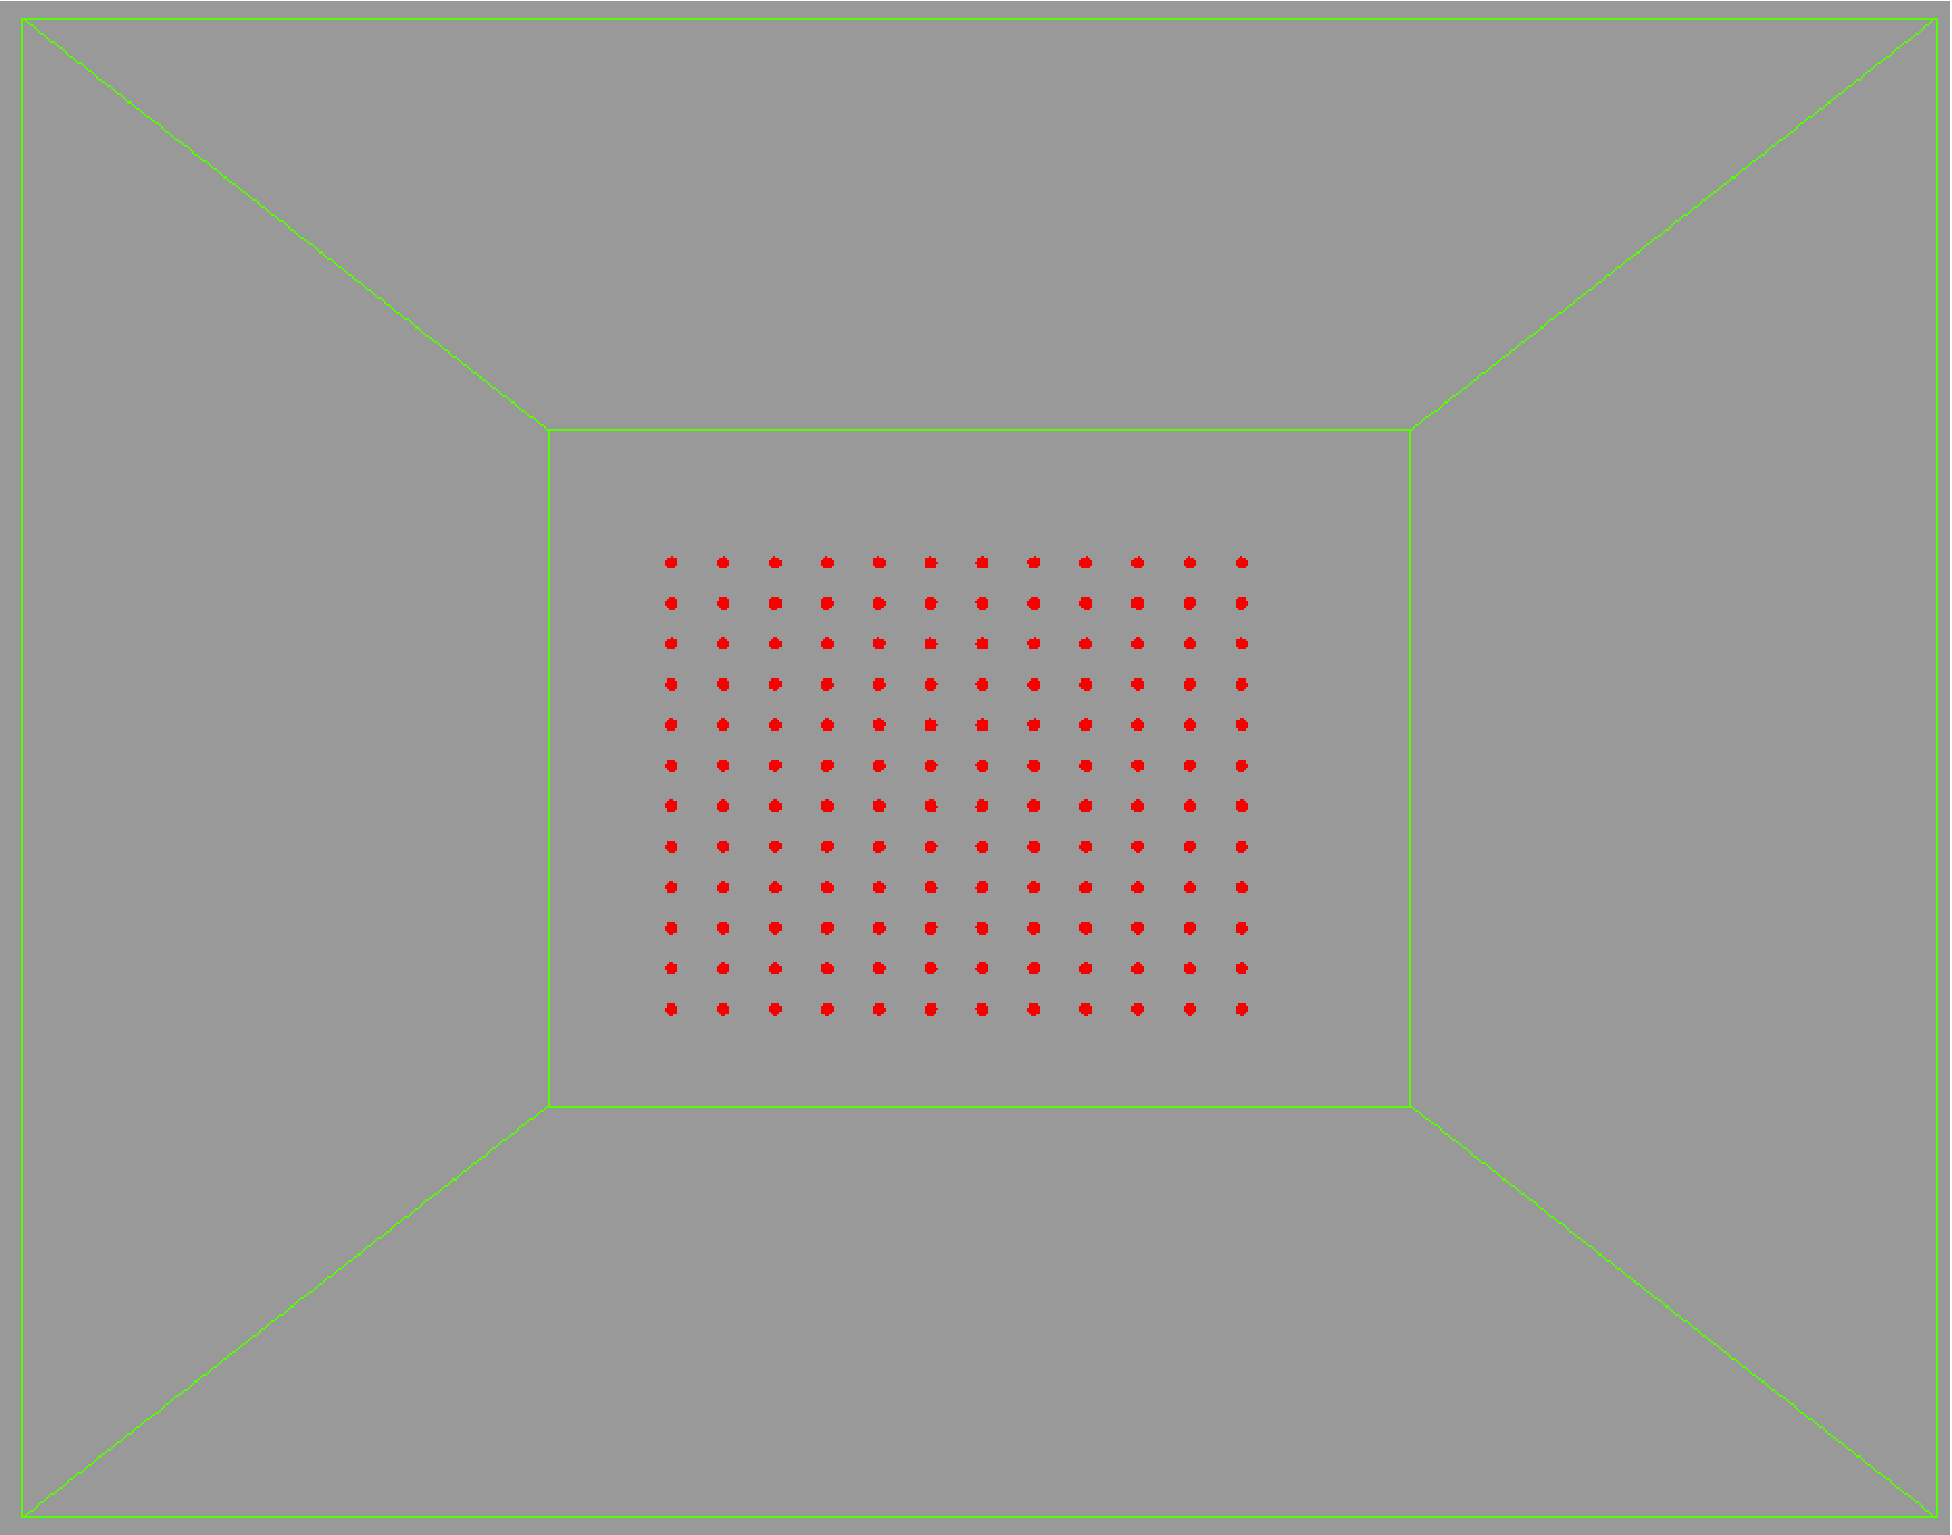
\includegraphics[scale=0.15]{figures/align.pdf}
\caption{Initial state of the boids}
\label{alignRule}
\end{center}
\end{figure}

% separation
\begin{figure}[htbp]
\begin{center}$
\begin{array}{cc}
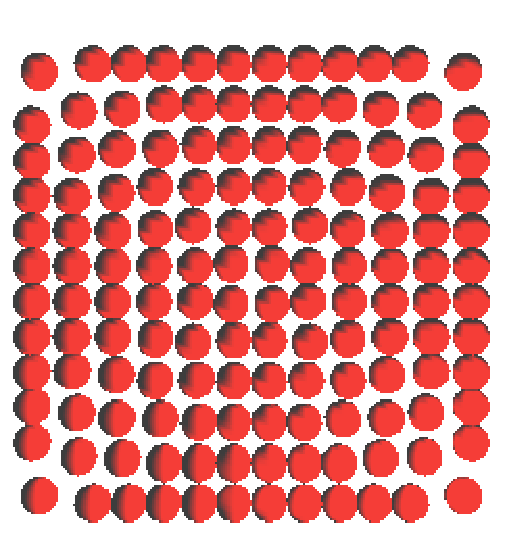
\includegraphics[scale= 0.15]{figures/sep1.pdf} &
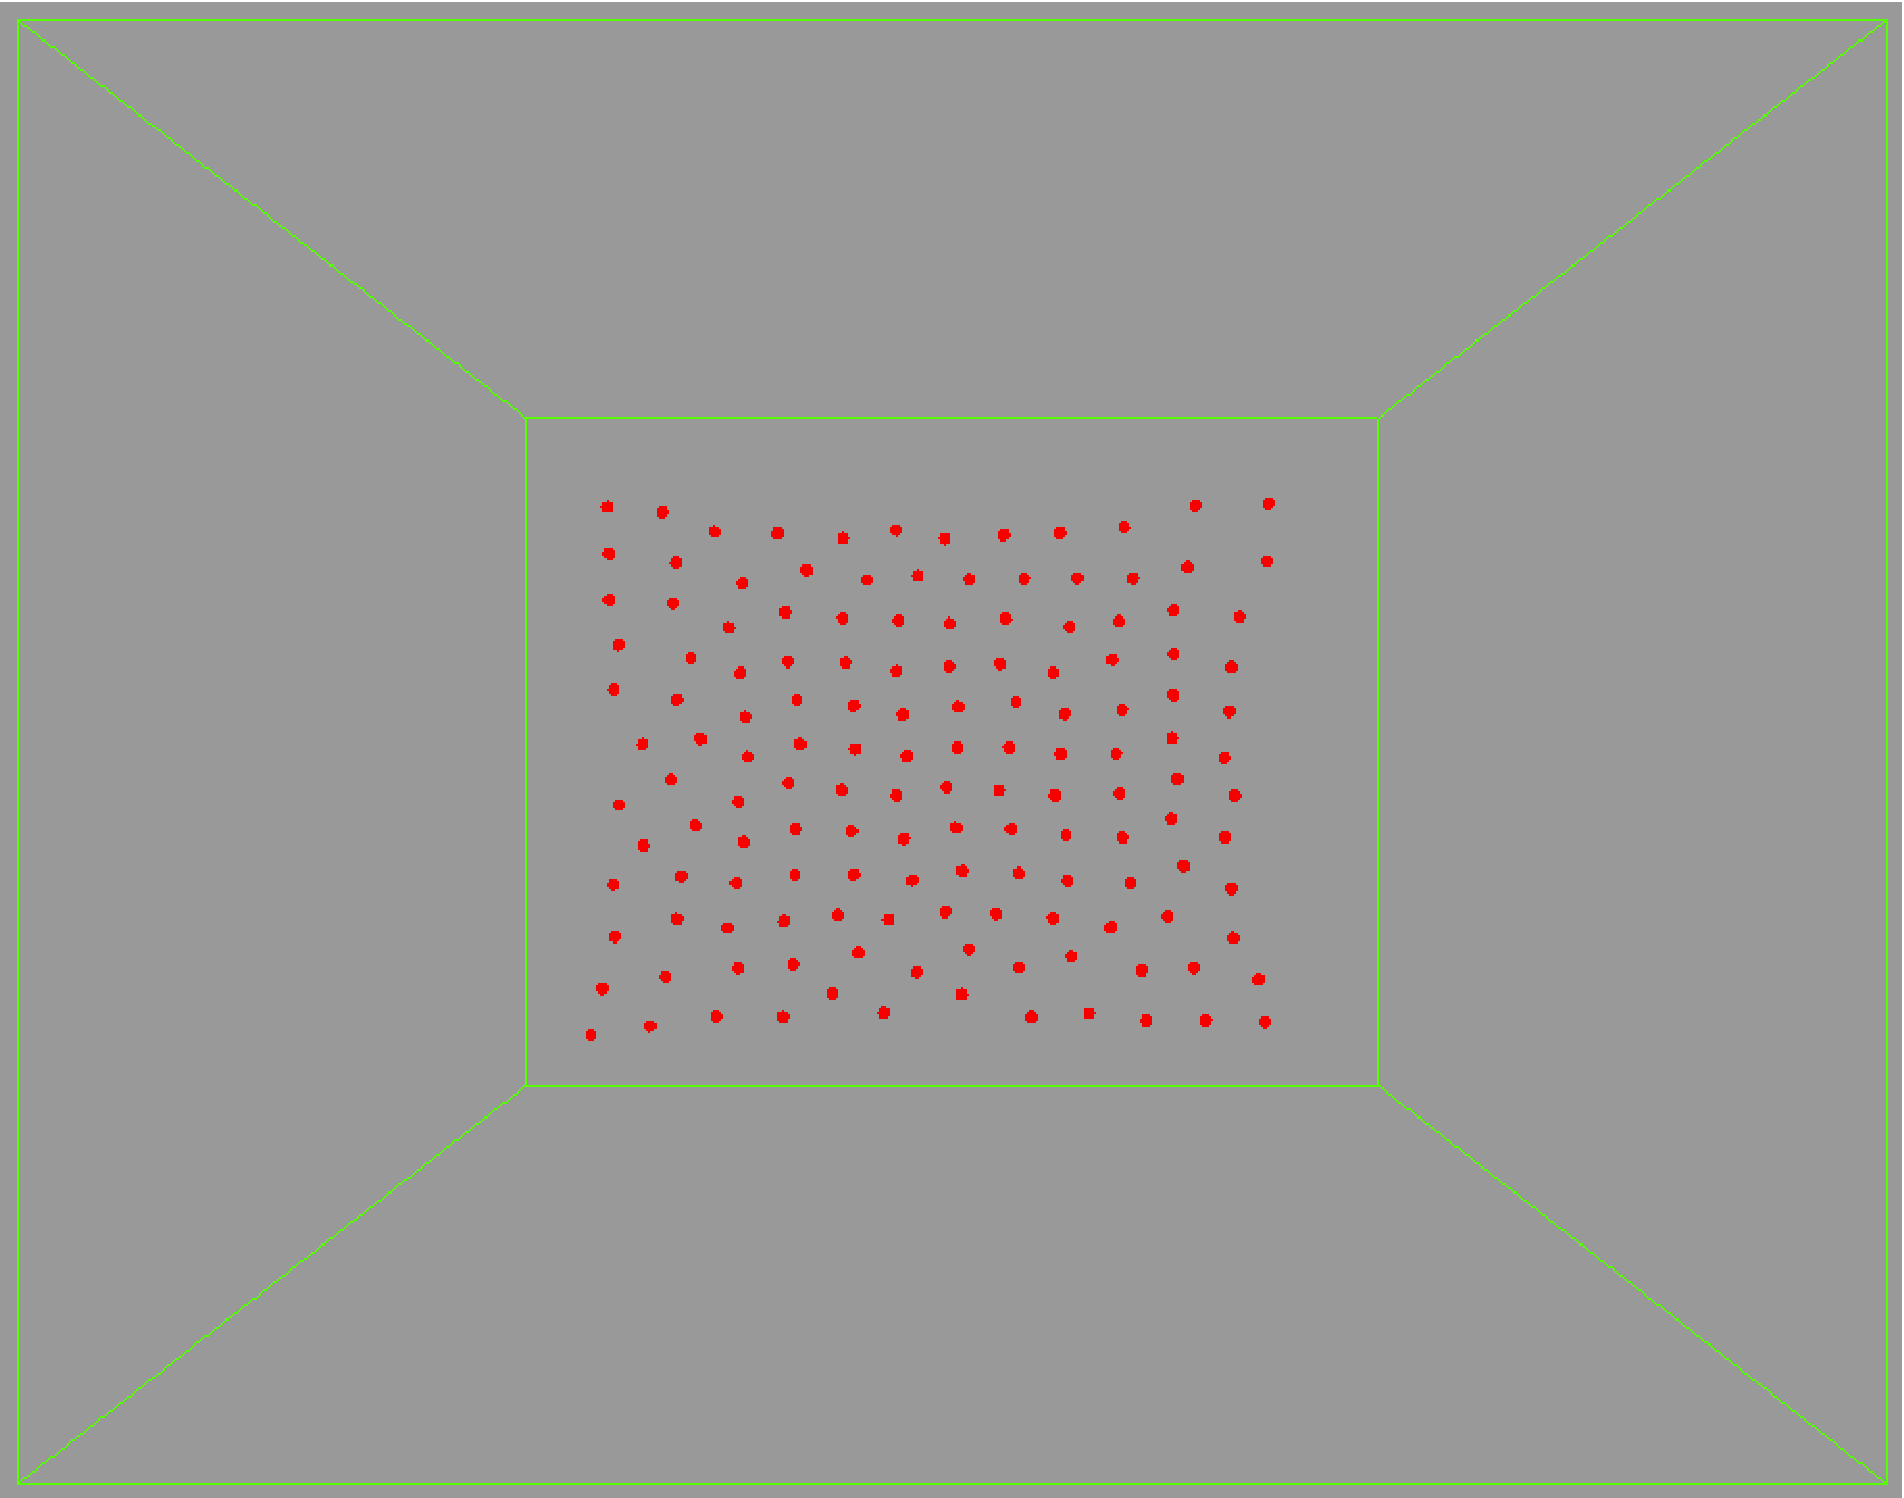
\includegraphics[scale= 0.15]{figures/sep2.pdf}
\end{array}$
\end{center}
\caption{Screenshots of the separation rule}
\label{sepRule}
\end{figure}

% cohesion
\begin{figure}[htbp]
\begin{center}
\begin{tabular}{cc}
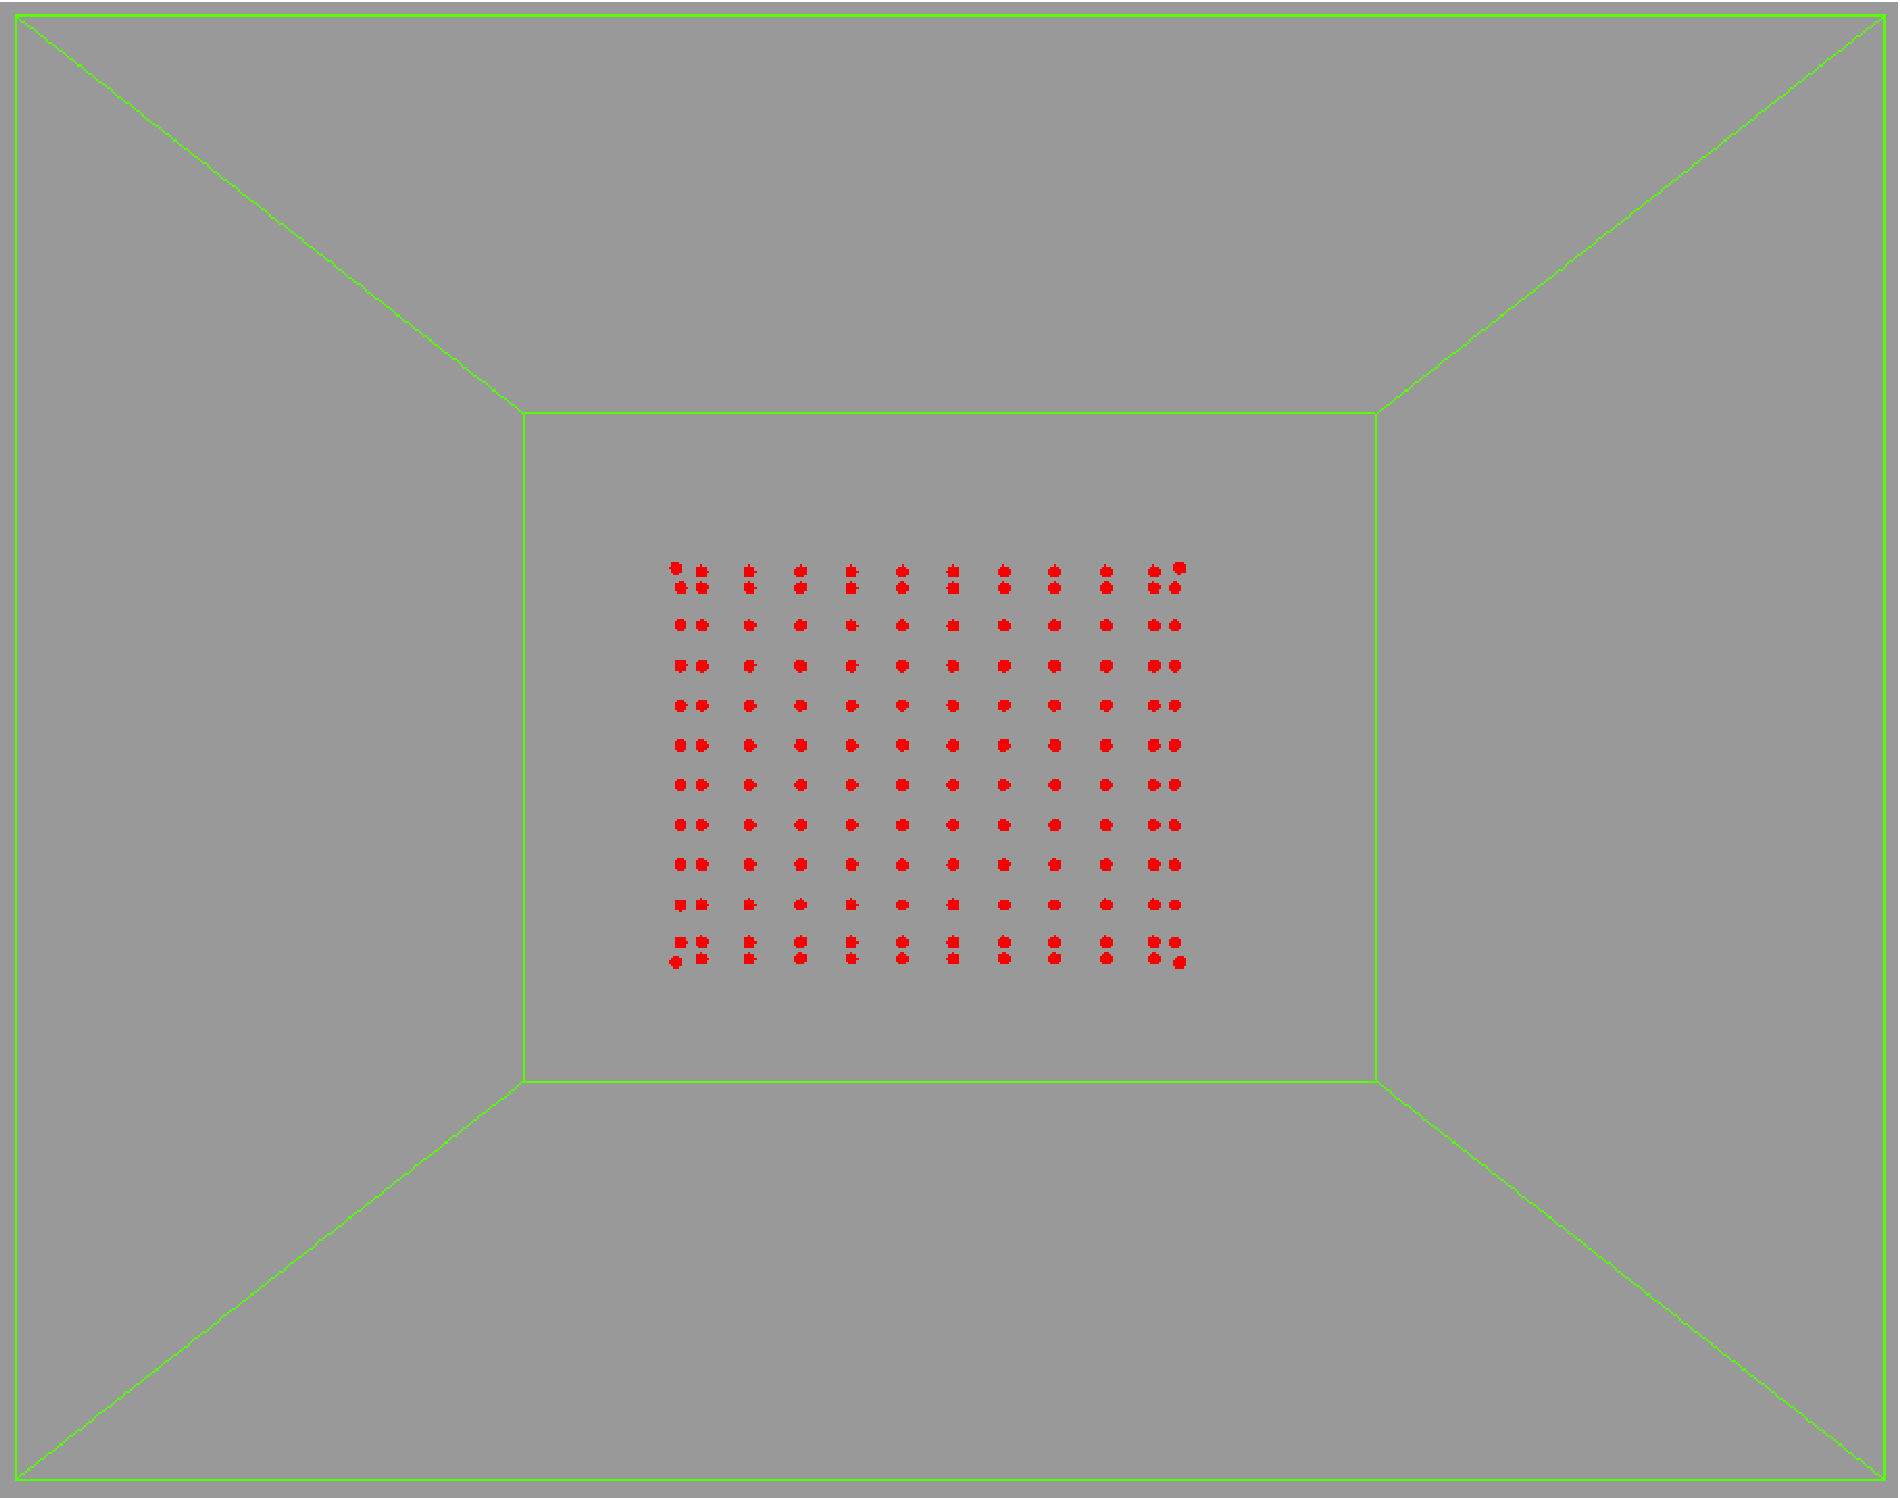
\includegraphics[scale= 0.15]{figures/coh1.pdf} &
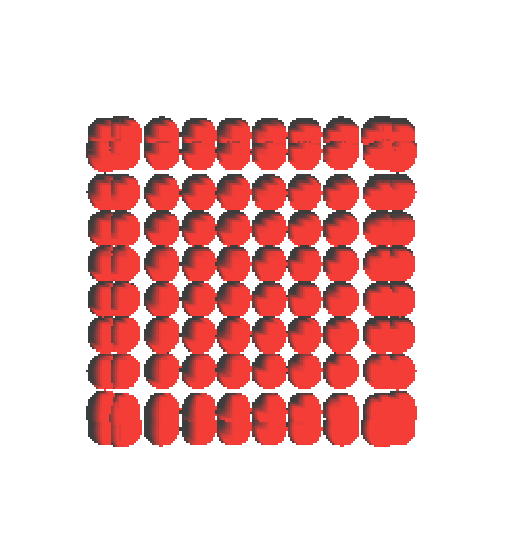
\includegraphics[scale= 0.15]{figures/coh2.pdf} \\

\includegraphics[scale= 0.15]{figures/coh3.pdf} &
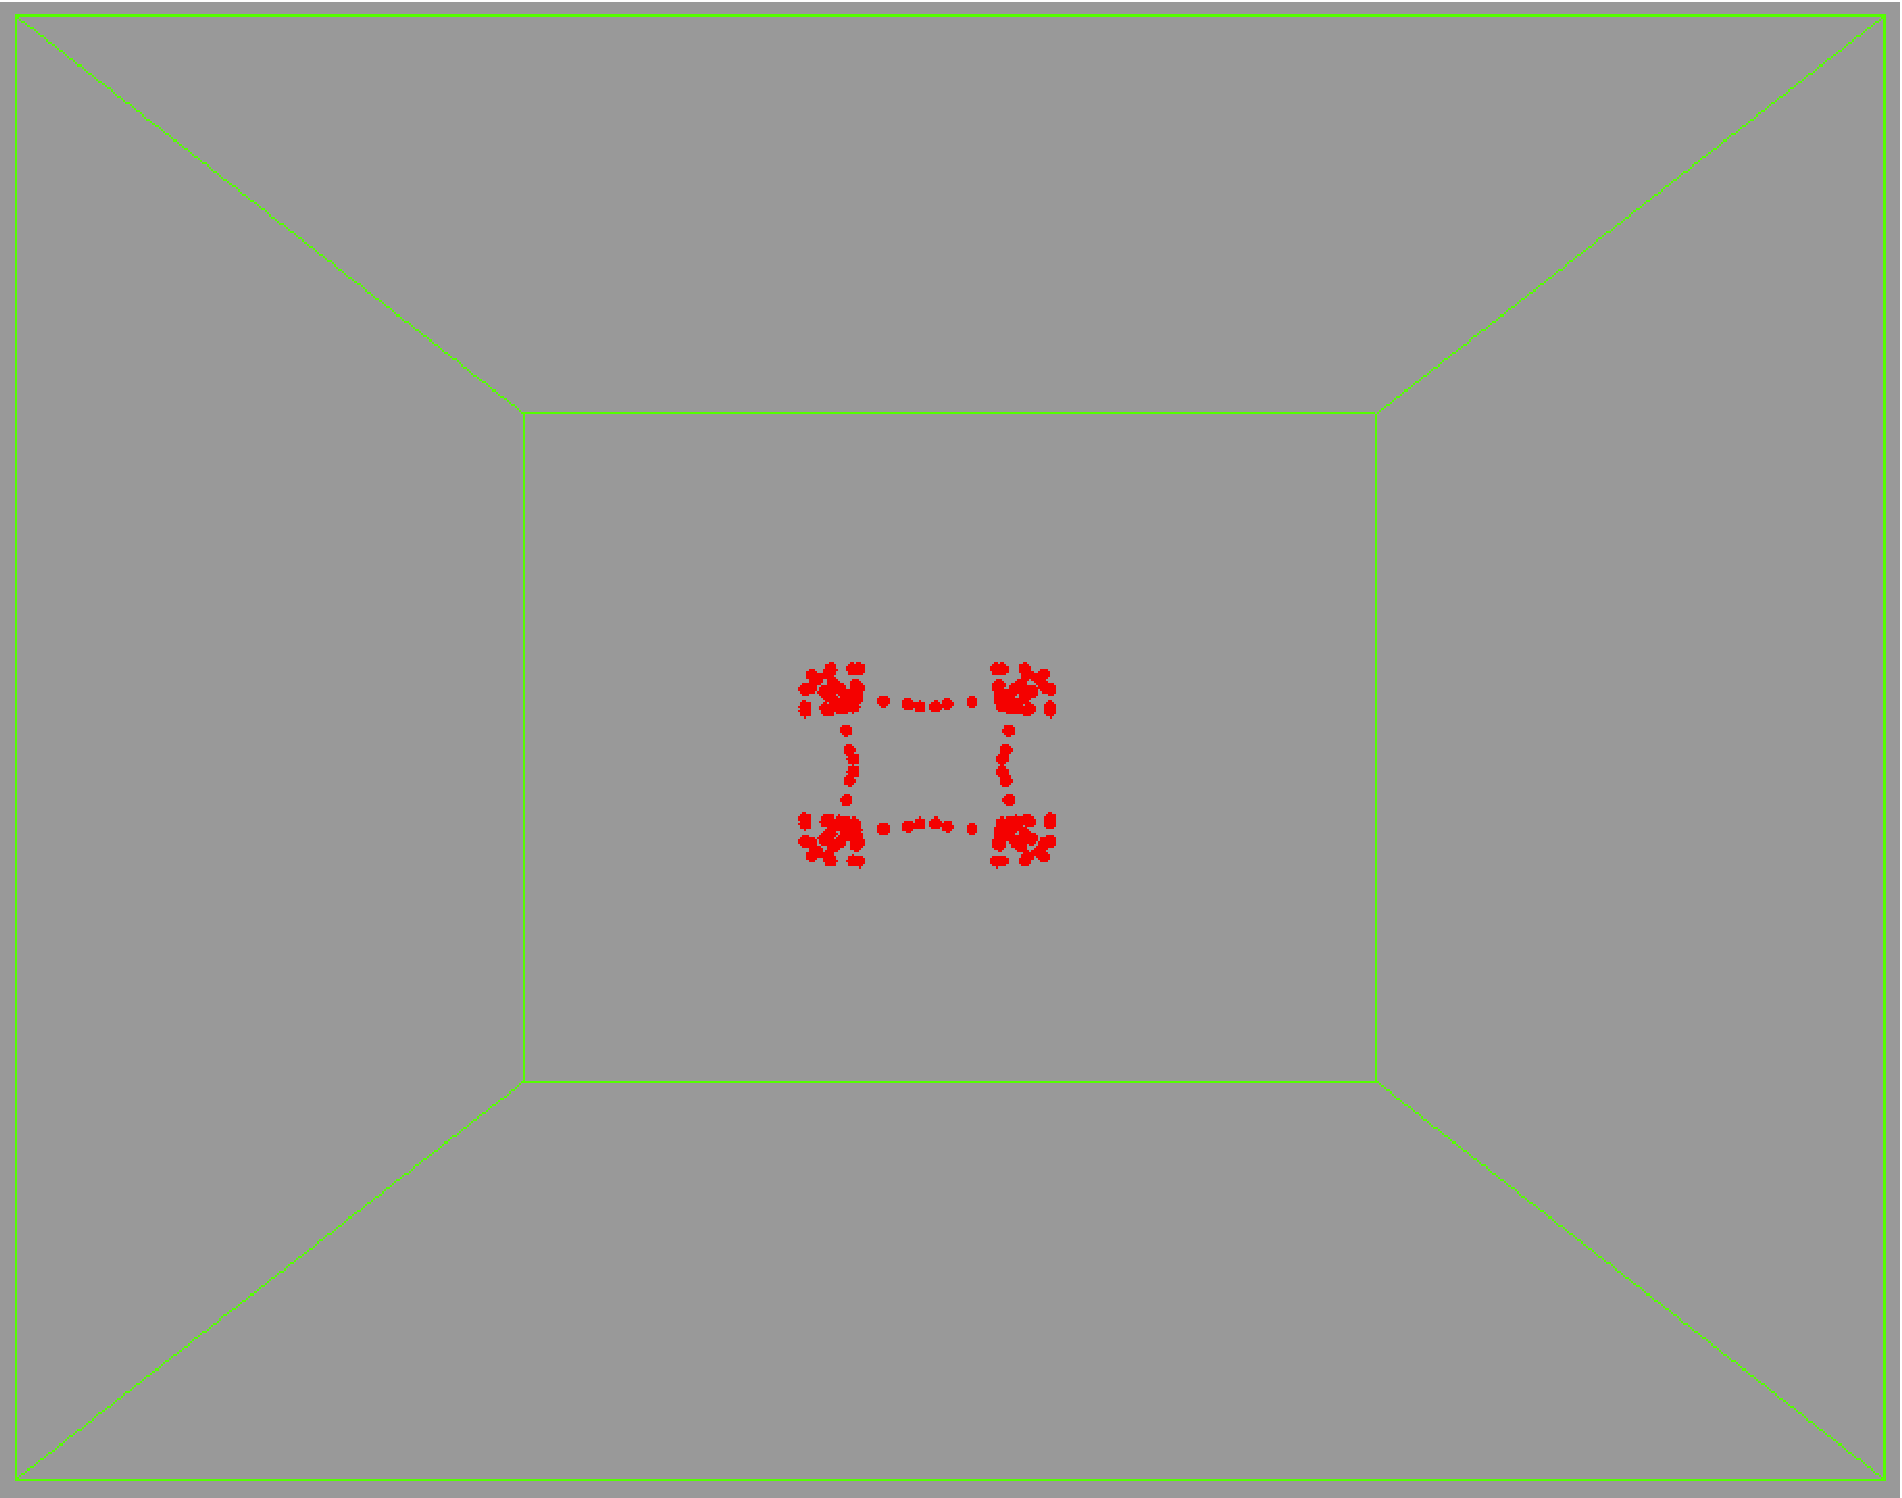
\includegraphics[scale= 0.15]{figures/coh4.pdf}
\end{tabular}
\end{center}
\caption{Screenshots of the cohesionrule}
\label{cohRule}
\end{figure}

\subsection{Blender Demo}
\textcolor{red}{** TODO: missing the Blender demo ***}

\section{Benchmarks}
% mention which kind of hardware I'm using

The flocking OpenCL implementation presented in this thesis seems to outperform Blender Boid system. Figure~\ref{plot} show the timings for up to more than half of a million boids. This boids were represented as spheres in a simple scene with no other objects. Blender was running faster than RTPS when the amount of particles were small, then when big numbers came around, Blender's performance disappear.  We were able to render more than $65K$ boids at $60$ fps and more than half of a million boids at a rate of $10$ fps.

\begin{figure}[htbp]
\begin{center}
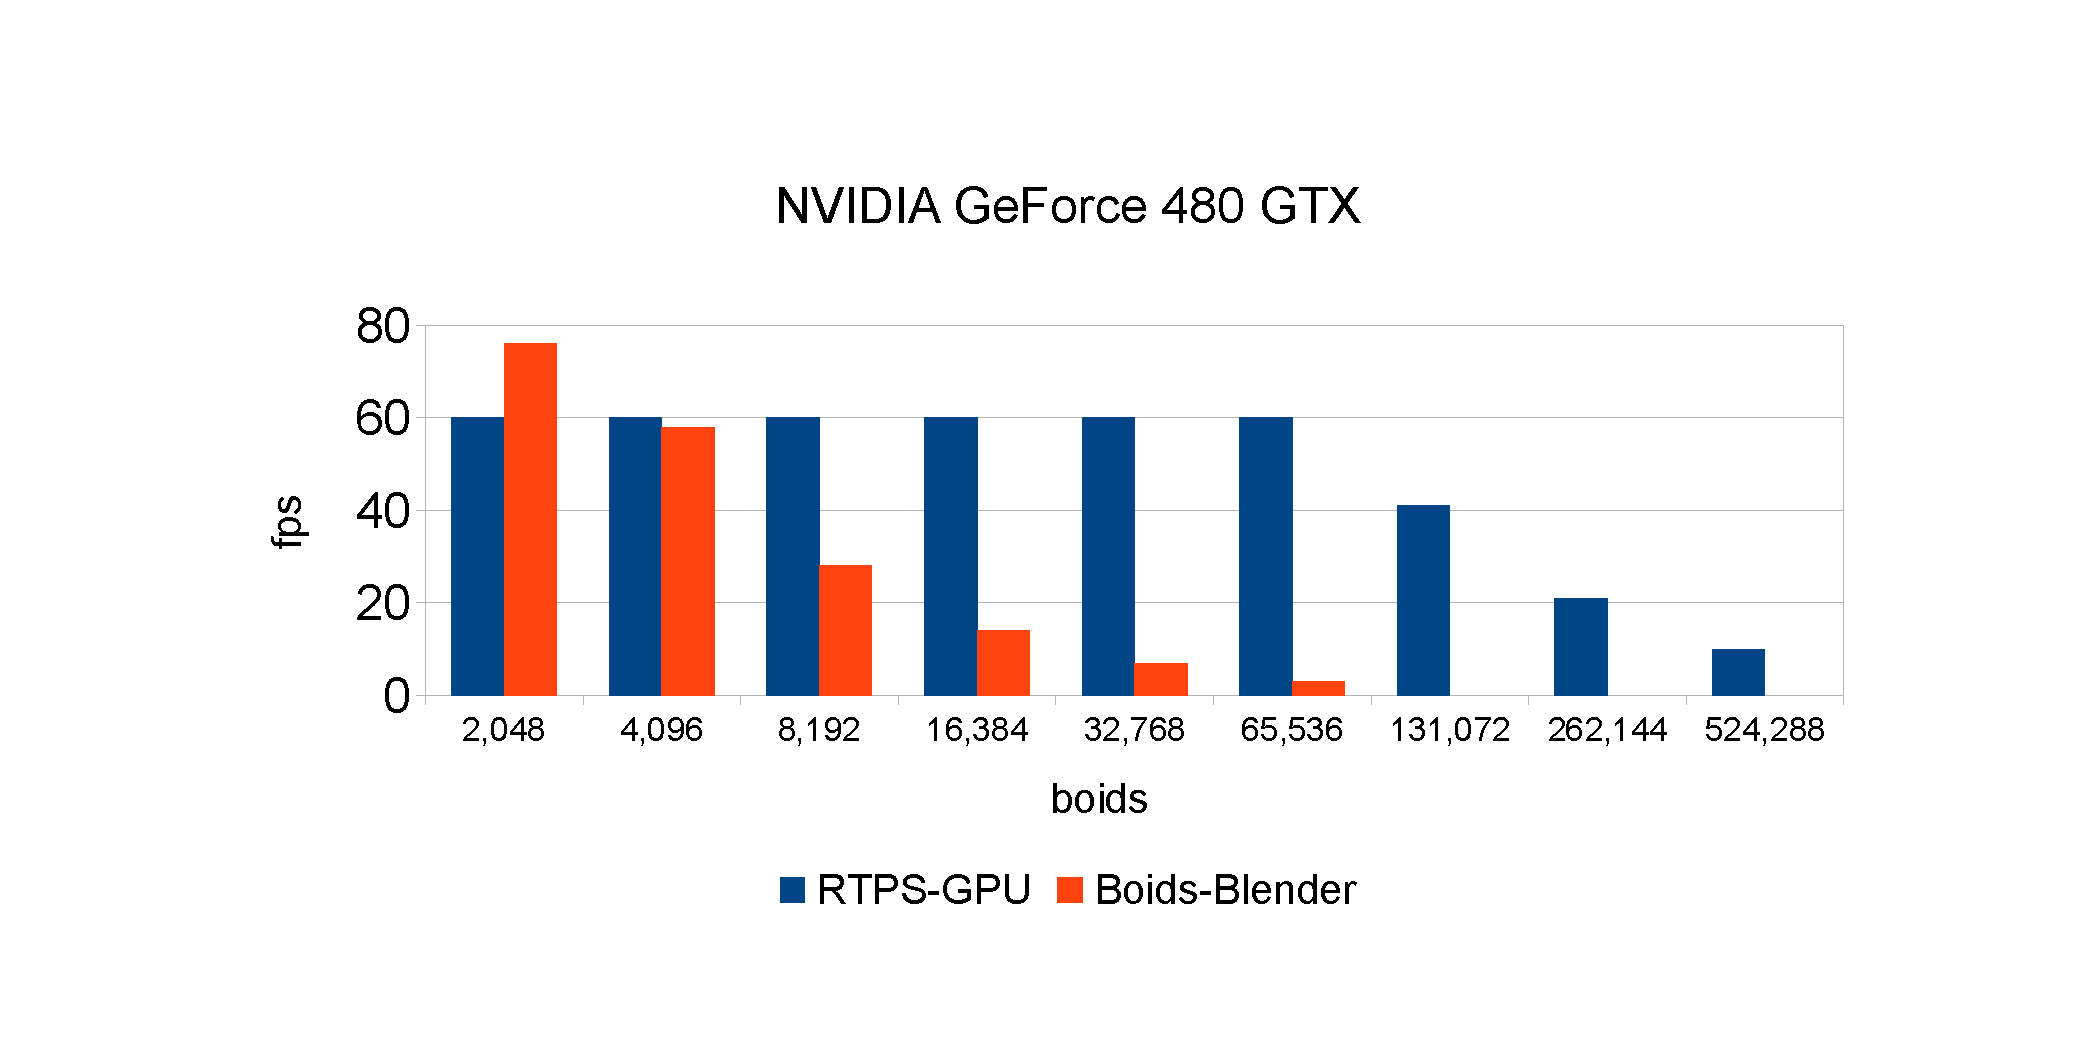
\includegraphics[scale=0.45]{figures/benchmarks.pdf}
\caption{Timings of RTPS modifier and Blender Boids system}
\label{plot}
\end{center}
\end{figure}

Comparing our performance with some of the statistics that were mentioned in Section~\ref{flockingGPU}, our flocking implementation still outperforming. The library BehaveRT was used to run simulations in real-time and visualization, Era et al. ran $130K$ boids at 15 fps, we ran more than $131K$ boids at 41 fps. Of course, it also depends on which hardware they used to get the benchmarks. Our benchmarks were taken in a Dell XXX with a processor XXX, XXX of memory and a NVIDIA GeForce 480 GTX GPU computing device. 

We also measure the inner performance of RTPS, to do so, we measure the time that took every kernel to be executed. Figure~\ref{kernelBench} shows the timings for the kernels.

\textcolor{red}{TODO: create a chart with the timings per kernel}



